%%=============================================================================
%% Conclusie
%%=============================================================================

\chapter{Conclusie}
\label{ch:conclusie}

\section{Waargenomen verbeteringen door gebruik te maken van een toewijzing met CSP}
Figuur \ref{grafiek:gemiddeld-service-level} geeft een spreiding weer van het gemiddelde service level voor de gesimuleerde druktegraden voor zowel de eenvoudige toewijzing als voor de toewijzing met het algoritme. 
\begin{figure}[h]
	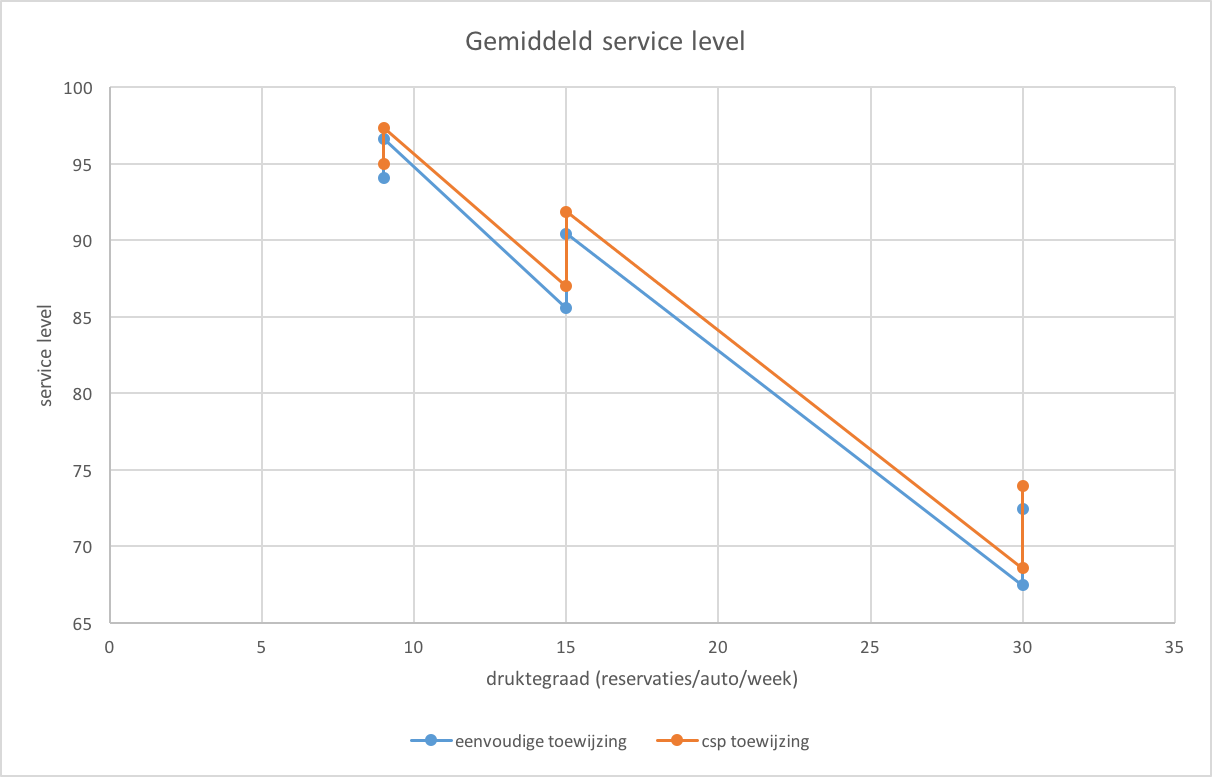
\includegraphics[width=\textwidth]{grafiek-gemiddeld-service-level.png}
	\caption[Grafiek van het gemiddelde service level per druktegraad]{Grafiek van het gemiddelde service level per druktegraad}
	\label{grafiek:gemiddeld-service-level}
\end{figure}
Figuur \ref{grafiek:gemiddelde-tijd-actief-per-auto} geeft een spreiding weer voor de gemiddelde tijd actief per auto voor de gesimuleerde druktegraden voor zowel de eenvoudige toewijzing als voor de toewijzing met behulp van CSP's.
\begin{figure}[h]
	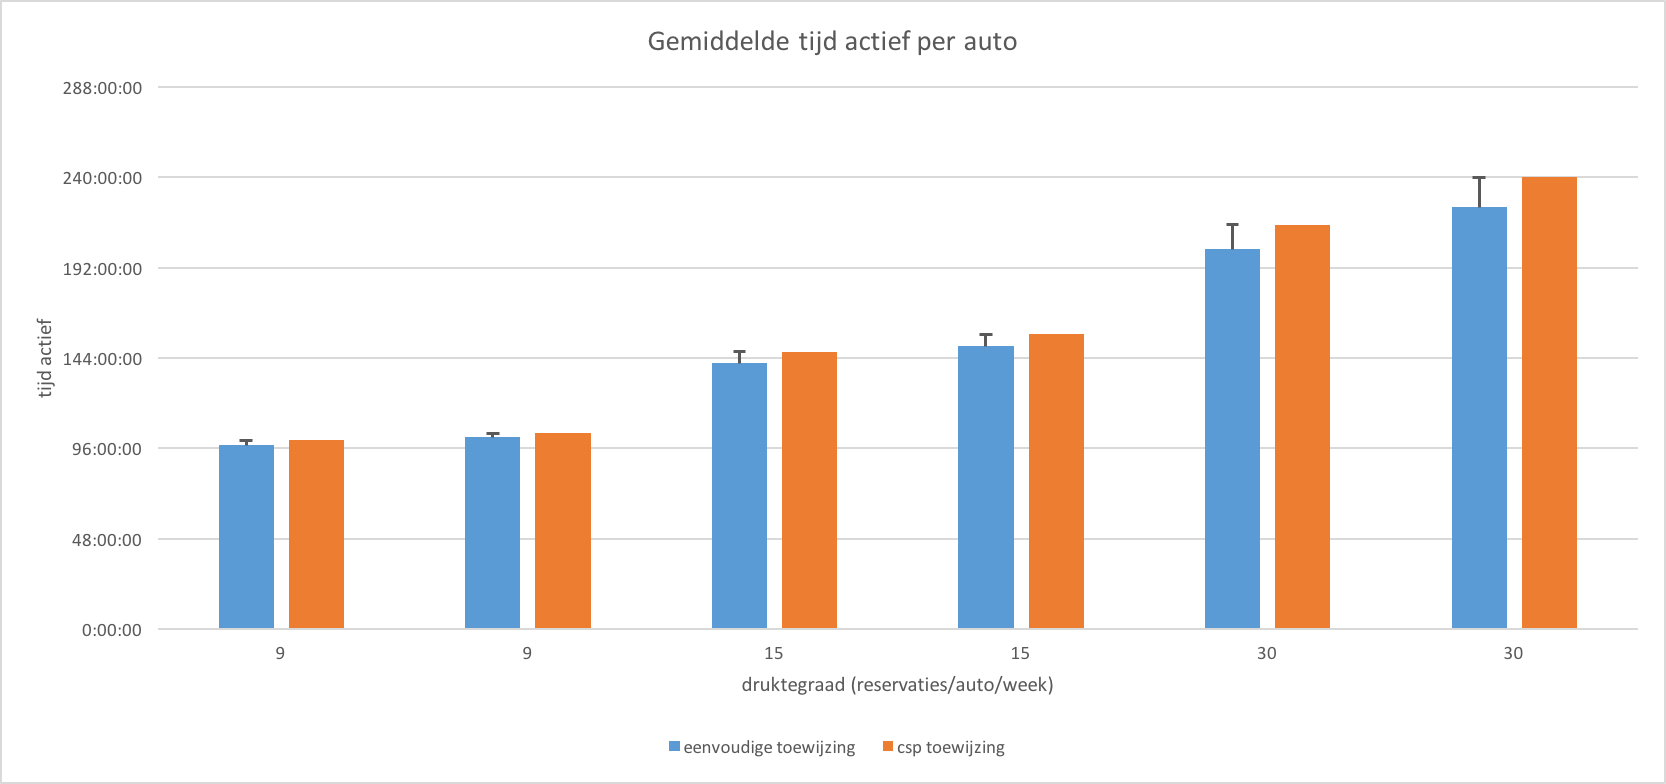
\includegraphics[width=\textwidth]{grafiek-gemiddelde-tijd-actief-per-auto.png}
	\caption[Grafiek van de gemiddelde tijd actief per auto per druktegraad]{Grafiek van de gemiddelde tijd actief per auto per druktegraad}
	\label{grafiek:gemiddelde-tijd-actief-per-auto}
\end{figure}
In figuur \ref{grafiek:gemiddeld-service-level} kan reeds in één oogopslag de meest voor de hand liggende conclusie getrokken worden: het service level voor de toewijzing met het csp algoritme ligt steeds hoger dan de eenvoudige toewijzing. De winstmarges die geboekt worden door gebruik te maken van CSP's is echter klein. Over alle simulaties heen werd er een gemiddelde verhoging van 1,2\% van het service level waargenomen. Figuur \ref{grafiek:gemiddelde-verbetering-service-level} geeft de gemiddelde verbetering voor het service level weer voor de verschillende druktegraden voor de simulaties met 3 auto's (blauw) en 5 auto's (oranje)
\begin{figure}[h]
	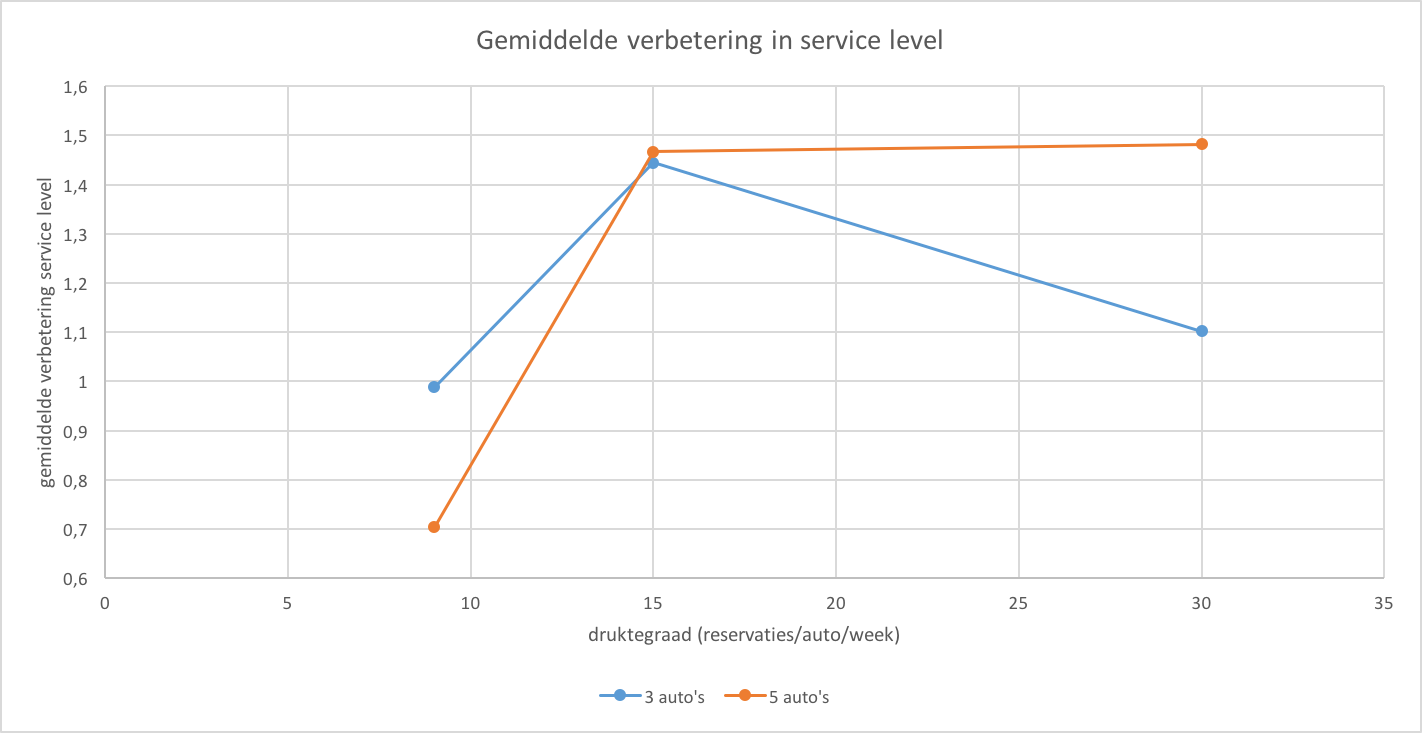
\includegraphics[width=\textwidth]{grafiek-gemiddelde-verbetering-service-level.png}
	\caption[Grafiek van de gemiddelde verbetering van het service level]{Gemiddelde verbetering van het service level met 3 en 5 auto's}
	\label{grafiek:gemiddelde-verbetering-service-level}
\end{figure}
Uit deze grafiek blijkt dat de verbeteringen voor hogere druktegraden wel hoger lijken te liggen. Voor een druktegraad van 9 reservaties per week per auto wordt er een gemiddelde verbetering van het service level van 0,99 en 0,7 gemeten. Voor een druktegraad van 15 reservaties per week per auto wordt er reeds een verhogen van 1,44 en 1,47 gemeten van het service level. Hoe complexer het probleem, met andere woorden, hoe meer auto's en hoe drukker het systeem, hoe groter de mogelijke winstmarges lijken. Dit wordt tevens ook weergegeven in figuur \ref{grafiek:gemiddelde-tijd-actief-per-auto}. De simulaties met hogere druktegraad, rechts in de figuur, vertonen een groter verschil tussen de blauw kolom (de eenvoudige toewijzing) en de oranje kolom (de toewijzing met behulp van CSP's). Deze conclusie kan echter niet met zekerheid getrokken worden. Er zouden nog meer simulaties uitgevoerd moeten worden met hogere druktegraden en meer auto's. (zie ook \ref{beperkingen-onderzoek}). De gemeten gemiddelde verbetering van het service voor druktegraad 30 met 3 auto's lijkt dit ook tegen te spreken. Aangezien de gemiddelde verbetering voor het service level terug daalt ten opzichte van de simulatie voor druktegraad 15 met 3 auto's. De simulaties voor 3 auto's met druktegraad 30 werden een extra keer uitgevoerd, maar gelijkaardige resultaten deden zich voor. De gemiddelde tijd actief per auto voor deze simulatie is echter wel consistent met deze bewering. 
De gemiddelde tijd actief per auto ligt voor de toewijzing met CSP steeds hoger dan voor de eenvoudige toewijzing. Dit wordt weergegeven in figuur \ref{grafiek:gemiddelde-tijd-actief-per-auto} 
Figuur \ref{grafiek:gemiddelde-verbetering-tijd-actief} toont de gemiddelde verbetering van de tijd dat een auto actief was voor 3 en 5 auto's. Deze grafiek ondersteund de bewering dat hoe complexer het probleem het groter de winstmarge. De rechte die de data voor 5 auto's verbindt stijgt immers steiler dan die voor 3 auto's.
\begin{figure}[h]
	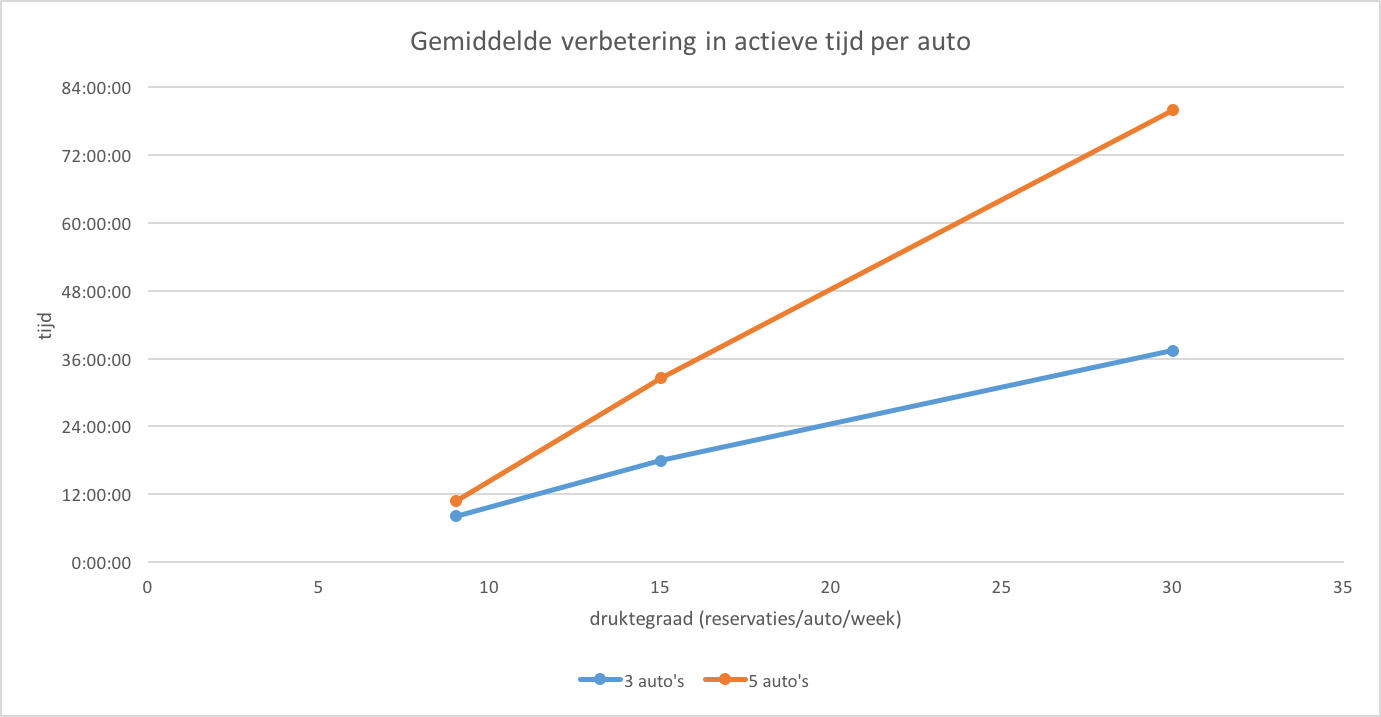
\includegraphics[width=\textwidth]{grafiek-gemiddelde-verbetering-tijd-actief-per-auto.png}
	\caption[Grafiek van de gemiddelde verbetering van de tijd actief per auto]{Gemiddelde verbetering van de tijd actief per auto voor 3 en 5 auto's}
	\label{grafiek:gemiddelde-verbetering-tijd-actief}
\end{figure}

\section{Antwoord op de onderzoeksvraag}
De onderzoeksvraag die geformuleerd werd in het begin van deze onderzoekstekst luidde als volgt: ``Stijgt het service level en de gebruiksduur van de auto's van Partago  wanneer de gebruikers geen specifieke auto's reserveren, maar enkel een zone?'' Vertaalt naar hoe dit onderzoek gevoerd werd: stijgt het service level en de gebruiksduur van de auto's van Partago met een toewijzing die gebruik maakt van CSP's ten opzichte van een eenvoudige toewijzing. Als de onderzoeksvraag als een ja-nee vraag geïnterpreteerd wordt dan is het antwoord ``ja''. De gemeten verbeteringen voor zowel het service level als voor de tijd actief per auto zijn echter relatief klein. In het prijsmodel van Partago is de gereserveerde tijd één van de factoren die de prijs van een rit bepaald. Het is dan ook nuttig om de auto's actiever te maken, ook al is dit maar een beetje. In het huidige prijsmodel is de gemiddelde kostprijs 3euro/uur voor de gebruiker. Afhankelijk van de druktegraad kan er dus per auto wel meer verdiend worden. Of de financiële winst dat dit met zich meebrengt opweegt ten opzichte van de kost dat het met zich zou meebrengen om het platform hieraan aan te passen is een oefening die in dit onderzoek moeilijk gemaakt kan worden, maar met de relatief kleine gemiddelde winstmarge van 1,2\% voor het service level wordt een voorzichtige ``nee'' geformuleerd op deze vraag. Moest uit verder onderzoek blijken dat de winstmarges hoger worden bij een nog drukker systeem zoals ook gesuggereerd in dit onderzoek dan wordt het in de verre toekomst voor Partago misschien wel nuttig. Verder onderzoek zal dit moeten uitsluiten.

\section{Beperkingen van dit onderzoek en een aanzet tot verder onderzoek} \label{beperkingen-onderzoek}
De eerst grote beperking is het relatief kleine aantal datapunten die gebruikt zijn in dit onderzoek. De originele opzet met het uitvoeren van simulaties met zelf geschreven code was om een groot aantal datapunten te kunnen genereren voor een zeer diverse set van parameters van de simulaties. De simulatietool gebruikt in dit onderzoek is geschreven in Dart, net zoals de rest van het Partago-platform. Voor de programmeertaal Dart bestaat er echter slechts 1 bibliotheek voor het oplossen van CSP's. Deze software-bibliotheek is een zeer eenvoudige en niet-performante implementatie zonder gebruik van de verschillende optimalisatiemogelijkheden zoals heuristieken. Hierdoor liep de rekentijd exponentieel op naarmate het probleem complexer werd. De rekentijd voor de uitgevoerde simulaties in dit onderzoek ligt nu reeds op meer dan 100 uur. Verder onderzoek zou dit onderzoek kunnen herhalen, maar om het CSP op te lossen gebruik maken van meer performante manieren zoals de OptaPlanner gerefereerd in het onderzoeksvoorstel van dit onderzoek. Moest Partago deze aanpak ooit naar de praktijk willen brengen moeten de CSP's zeer snel opgelost kunnen worden. Vanaf er een reservatie bijkomt moet er immers voor alle toekomstige reservaties van die dag een nieuwe mogelijjke toewijzing gedaan worden. Een rekentijd van enkele uren is dan niet aanvaardbaar. 
Een tweede grote beperking van dit onderzoek is dat voor de toewijzing van een auto aan een reservering er vanuit werd gegaan dat alle reservaties voor de dag gekend zijn voor de start van de eerste reservatie. In de simulatie wordt op dit tijdstip het Constraint Satisfaction Problem opgelost. In de praktijk komen er gedurende de dag echter nog reservaties bij of is er zelfs spontaan gebruik: mensen die een reservatie maken om dan 5 minuten later gebruik te maken van de auto. Momenteel wordt er in het onderzoek geen rekening gehouden met het tijdstip waarop de reservatie gemaakt werden. Deze informatie bevindt zich echter wel in de originele dataset van historische Partago-reservaties. Verder onderzoek zou wel kunnen gebruik maken van dit dataveld. Reservaties die reeds gestart of gepasseerd zijn op de moment van toekomen van een reservatie mogen dan geen deel meer uitmaken van het CSP probleem. 

